\documentclass[aspectratio=169]{beamer}

\usepackage{makecell}
\usepackage{booktabs}

\usetheme{Boadilla}

\title{Epidemic Broadcast}
\subtitle{Performance Evaluation of Computer Systems and Networks}
\author[Abdulwahed, Cima, Scatena]{Ahmed Khalil A. Abdulwahed, Lorenzo Cima, Niccolò Scatena}
\institute[UNIPI]{University of Pisa}
\date{2020/2021}

\begin{document}

\begin{frame}
	\titlepage{}
\end{frame}

\section{Simulation model}

\begin{frame}{The model}
	\begin{columns}
		\column{0.6\textwidth}
		\begin{itemize}
			\item 2D floorplan with users randomly dropped in
			\item A random user sends out a message; the other users
				relay it with a broadcast radius \emph{R}
			\item Time is \emph{slotted}
			\item \textbf{Trickle relaying}: when a user receives a
				message, it waits for \(T\) slots: message
				relayed if less than \(m\) copies received
		\end{itemize}
		\column{0.35\textwidth}
		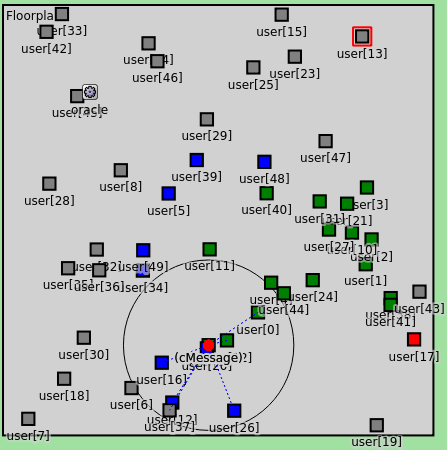
\includegraphics[width=\textwidth]{img/snapshot}
	\end{columns}
	Modules:
	\begin{description}
		\item[Floorplan] the network representing the 2D
			floorplan
		\item[User] submodule representing a user
		\item[Oracle] used to terminate simulation and collect
			some stats
	\end{description}
\end{frame}

\begin{frame}{User module}
	\begin{columns}
		\column{0.5\textwidth}
		Finite State Machine
		\begin{description}
			\item[IDLE] state when started; slotting through
				self-messages
			\item[RECEIVING] hearing message in current slot
			\item[COLLISION] received another message in the same
				slot
			\item[HEARING] waiting for time window \(T\)
			\item[RELAYING] relay message if trickle relaying not
				triggered
		\end{description}
		\column{0.5\textwidth}
		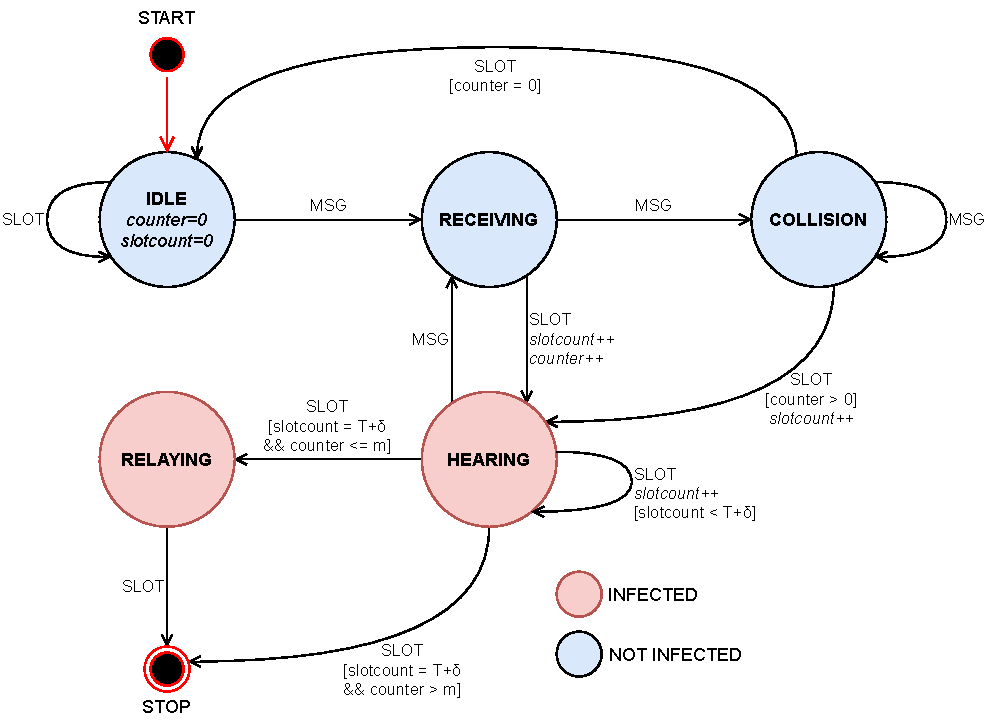
\includegraphics[width=\textwidth]{img/userfsm}
	\end{columns}
	User messages are sent with a duration equal to
	\(\frac{slotDuration}{2}\) in order to ensure that it is
	received in current slot
\end{frame}

\begin{frame}{Model verification}
	\begin{columns}
		\column{0.5\textwidth}
		\begin{description}
			\item[Valgrind] no memory leaks
			\item[Graphical] execution inside QTEnv
			\item[Step-by-Step Debug] code execution path
			\item[Event Trace] check for correct scheduling
			\item[Deterministic] same inputs \textrightarrow{} same outputs
			\item[Degeneracy] config with low params values
			\item[Continuity] input change \textrightarrow{} output
				change (figure)
		\end{description}
		\column{0.5\textwidth}
		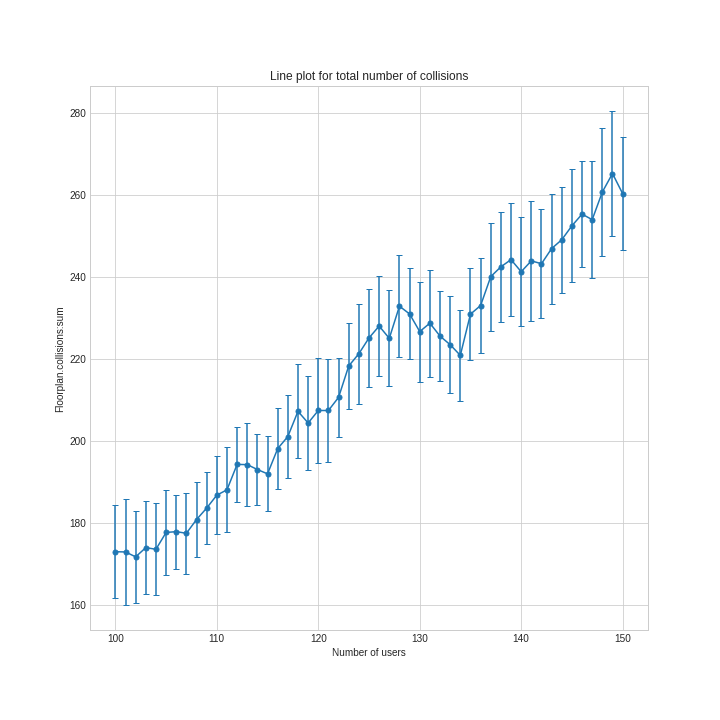
\includegraphics[width=\textwidth]{img/continuity-collisions}
	\end{columns}
\end{frame}

\section{Experiments design}

\begin{frame}{Factors and Indexes}
	\begin{columns}
		\column{0.5\textwidth}
		Performance indexes:
		\begin{itemize}
			\item \textbf{Broadcast time} needed to cover a certain
				percentile of the users
			\item Final percentage of \textbf{covered users}
			\item \textbf{Energy efficiency}: depends on \(R\) and
				the number of messages sent
				\[\mathit{Eff} \propto \frac{1}{R \cdot M}\]
			\item \textbf{Collisions}
		\end{itemize}
		\column{0.5\textwidth}
		Tunable factors:
		\begin{itemize}
			\item Broadcast radius (\(R\))
			\item Trickle relaying hear window (\(T\))
			\item Trickle relaying max copies (\(m\))
			\item Maximum relay delay (\(\max(\delta)\)): introduced
				to avoid an issue with trickle relaying
		\end{itemize}
		Not tunable factors:
		\begin{itemize}
			\item Floorplan area (\(A\)) and dimensions ratio
				(\(\frac{X}{Y}\))
			\item User density (\(\frac{N}{A}\))
			\item Position of first user sending the message
		\end{itemize}
	\end{columns}
\end{frame}

\begin{frame}{Scenarios}
	\begin{columns}
		\column{0.65\textwidth}
		\begin{description}
			\item[High Density] \(A = 22500m^2\) (\(150m \times
				150m\)), \(N = 1125\mathit{users}\) (\(0.05
					\mathit{users}/m^2\))
			\item[Low Density] \(A = 250000m^2\) (\(500m \times
				500m\)), \(N = 1250\mathit{users}\) (\(0.005
					\mathit{users}/m^2\))
			\item[Rectangular] \(A = 30000m^2\) (\(300m \times
				100m\)), \(N = 1500\mathit{users}\) (\(0.05
					\mathit{users}/m^2\))
		\end{description}
		\column{0.35\textwidth}
		\begin{itemize}
			\item \(T \in [5s, 10s]\)
			\item \(\max(\delta) \in [5s, 10s]\)
			\item \(m \in [2, 6]\)
			\item \(R \in [30m, 50m]\) (low density)\\
				\(R \in [10m, 20m]\) (others)
		\end{itemize}
	\end{columns}
	\begin{block}{Analysis workflow}
		\(2^{k}r\) to spot most important factors for each index. Then,
		in-depth factorial analysis with the most important factors to
		study the behaviour between extreme values.
	\end{block}
	Jupyter notebooks: analysis automation
\end{frame}

\section{Data analysis}

\begin{frame}{High density (\(2^{k}r\))}
    \begin{columns}
		\column{0.5\textwidth}
		The coverage always reach high values (\(> 99\%\)), so we don't analyze it in these experiments

		\begin{table}
			\begin{tabular}{l | c | c}
				Parameter & Factor & Percentage \\
				\hline \hline
				Collisions & R & \(66.27\%\) \\
				& m & \(15.76\%\) \\
				\hline
				Messages & m & \(85.98\%\) \\
				\hline
				Broadcast Time & R & \(71.25\%\) \\
				& T & \(19.30\%\) \\
				\hline
			\end{tabular}
			\caption{Most influencing factors for parameters}
		\end{table}
		\column{0.5\textwidth}
		\begin{figure}
		    
\includegraphics[scale=0.3]{img/marchio_unipi_pant541}
		    \caption{Image Caption}
		\end{figure}
	\end{columns}
\end{frame}

\begin{frame}{High density (optimizations)}
%TODO
\end{frame}

\begin{frame}{Low density (\(2^{k}r\))}
	\begin{columns}
		\column{0.5\textwidth}
		Also in this case the coverage always reach high values (\(> 99\%\))

		\begin{table}
			\begin{tabular}{l | c | c}
				Parameter & Factor & Percentage \\
				\hline \hline
				Collisions & R & \(58.96\%\) \\
				& m & \(19.26\%\) \\
				\hline
				Messages & m & \(85.18\%\) \\
				\hline
				Broadcast Time & R & \(58.90\%\) \\
				& T & \(30.43\%\) \\
				\hline
			\end{tabular}
			\caption{Most influencing factors for parameters}
		\end{table}
		\column{0.5\textwidth}
		\begin{figure}
		    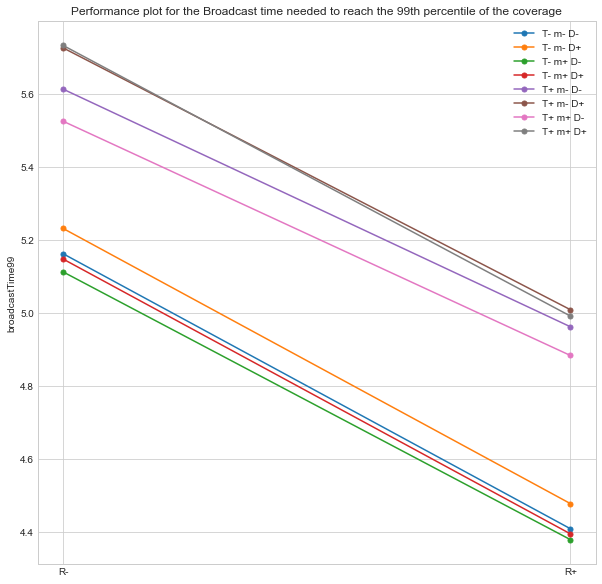
\includegraphics[height=0.65\textheight]{img/ld/broadcasttime-R-perfplot}
		    \caption{Increase R reduces so much the broadcast time (but increases the number of collisions and the energy consumed)}
		\end{figure}
	\end{columns}
\end{frame}

\begin{frame}{Low density (optimizations)}
	\footnotesize
	\begin{columns}
	    \column{0.5\textwidth}
	        \begin{itemize}
	        \item The minimum value of R to have a good coverage (\(> 99\%\)) is 25m
	        \item To improve energy efficiency, we never increase this broadcast radius for the parameter optimization study
	        \end{itemize}
	        \begin{center}
	            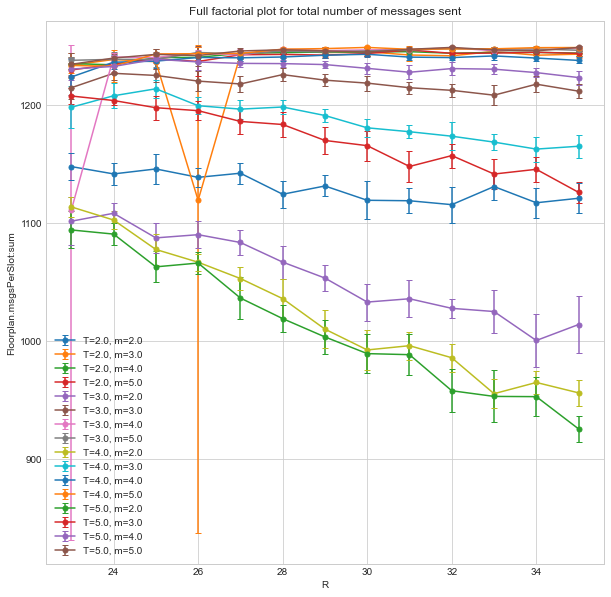
\includegraphics[width=0.7\textwidth]{img/ld/messages-R-ffplot.png}
	        \end{center}
	    \column{0.5\textwidth}
	        \begin{itemize}
	        \item A low number of max copies implies great benefits for all parameters
	        \item Trade-off between broadcast time and energy efficiency for the hear window parameter
	        \end{itemize}
	        \begin{center}
	            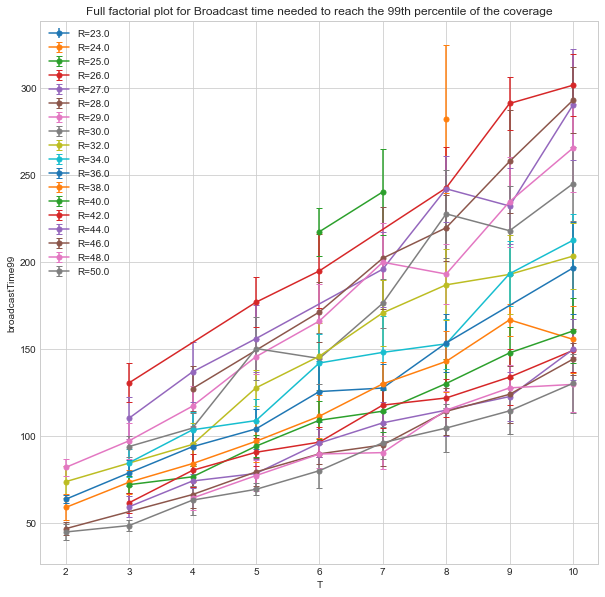
\includegraphics[width=0.7\textwidth]{img/ld/broadcasttime-T-ffplot.png}
	        \end{center}
	\end{columns}
\end{frame}

\begin{frame}{Rectangular floorplan}
		\begin{columns}
		\column{0.5\textwidth}
		 \begin{itemize}
		     \item
	Coverage almost always reaches 100\%.The lowest value is 99.6664\%. \\[5pt]

		\begin{table}
			\begin{tabular}{l | c | c}
				Parameter & Factor & Percentage \\
				\hline \hline
				Collisions & R & \(64.31 \%\) \\
				& m & \(16.47\%\) \\& Rm& \(9.59 \%\) \\
				\hline
				Messages & m & \(84.89\%\) \\& R & \(5.58\%\) \\
				\hline
				Broadcast Time & R & \(65.40\%\) \\
				& T & \(20.58\%\) \\
				\hline
			\end{tabular}
			\caption{Most influencing factors for parameters}
		\end{table}
		\item the shape of the plane has a negligible influence, so the obtained results for the optimizations are similar to previous ones
		\end{itemize}
		\column{0.5\textwidth}
				\begin{figure}
		    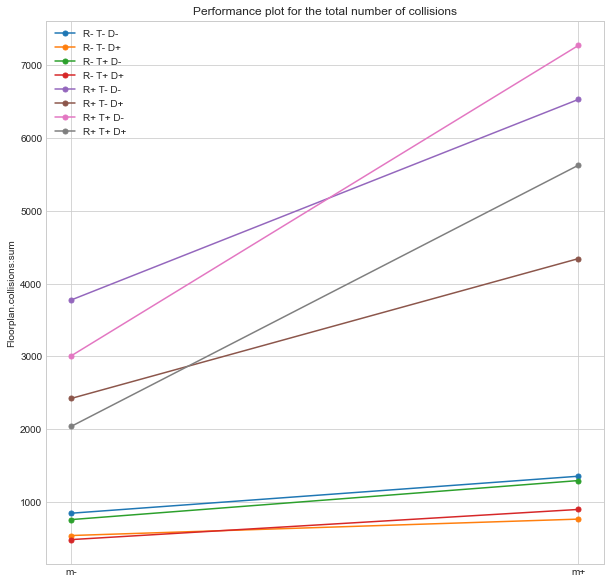
\includegraphics[height=0.65\textheight]{img/rect/collisions_m_perfplot.png}
		    \caption{Decrease the maximum number of copies to decrease the total
number of collisions}
		\end{figure}

	\end{columns}
\end{frame}

\begin{frame}{Position of starting node}
	\footnotesize
	\begin{columns}
		\column{0.5\textwidth}
		\footnotesize The broadcast time is so different changing the initial position of the first user. Note that, seeing the values in order of mean time, the maximum value for a starting position is always lower than the minimum of the following experiment, so the results are well defined
		\begin{table}
		\begin{tabular}{lcccc}
		\multicolumn{5}{c}{Low density (98th percentile broadcast time)}\\
		\toprule
		Start Node Pos\@. & Mean & Std\@. Dev\@. & Min\@. & Max\@. \\
		\midrule
		Center & \(35.166667s\) & \(1.533158s\) & \(31s\) & \(40s\) \\
		Border & \(53.7s\) & \(1.914554s\) & \(50s\) & \(58s\) \\
		Corner & \(65.1s\) & \(2.186952s\) & \(61s\) & \(70s\) \\
		\bottomrule
	    \end{tabular}
	    \end{table}
		\column{0.5\textwidth}
		    \begin{center}
		    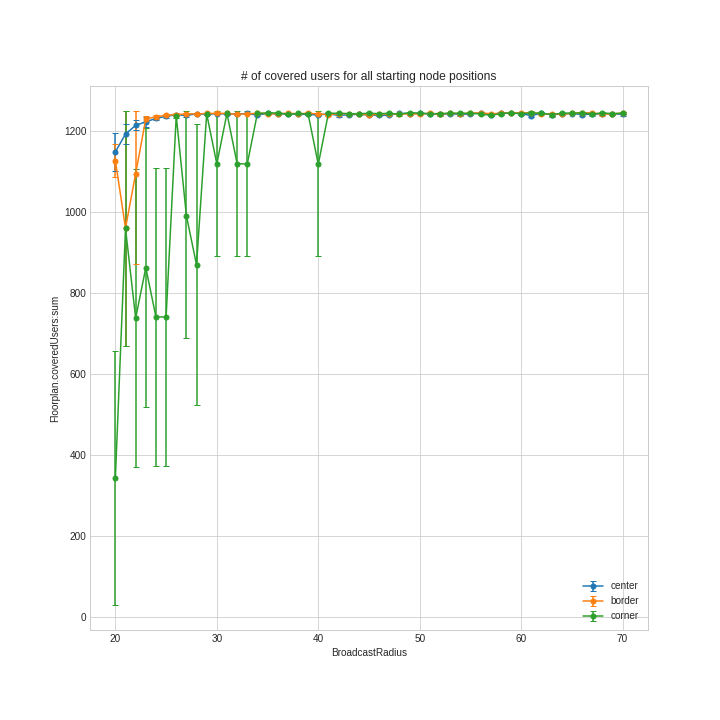
\includegraphics[height=0.75\textheight]{img/ld/start-node-coverage.png}
		    \end{center}
	\end{columns}
	\footnotesize The coverage has a similar mean for center and border starting points, but starting from the border we have also some situations where no users are reached. Starting from the corner we have many situations where no one is infected, this leads to a very large variance
\end{frame}

\section{Conclusions}

\begin{frame}{Conclusions}
\end{frame}

\begin{frame}
    \centering
    \Huge Thank you!
\end{frame}

\end{document}
